\setcounter{page}{1}

\section{Introducción}
\section{Objetivos}
    \begin{itemize}
        \item Emplear la herramienta \textbf{Wireshark} para realizar capturas y análisis de tráfico en una LAN.
        \item Analizar el comportamiento de los mandatos \textbf{ping} en una comunicación vía red.
    \end{itemize}
\section{Marco Teórico}
    Ejemplo de cita~(\cite{buffett84}).

\newpage
\section{Desarrollo del Trabajo}
    \textbf{Para esta práctica se requiere del uso de dos PC's (las denominaremos como PC1 y PC2), ambos equipos conectados por enlace directo y con IP's estáticas.}

    \subsection{Tarea 1.}
        \paragraph{Paso 1.}
        \textbf{Realice una tabla que contenga el nombre de cada equipo, su IP y su MAC.}

        Para comenzar, en la PC1 se inició con el sistema operativo \textbf{Windows} y se realizó el cambio de la dirección IP a \texttt{192.168.0.14} con la puerta de enlace \texttt{192.168.0.1}. Como se muestra en la Figura~\ref{fig:ip_windows}.

        \begin{figure}[H]
            \centering
            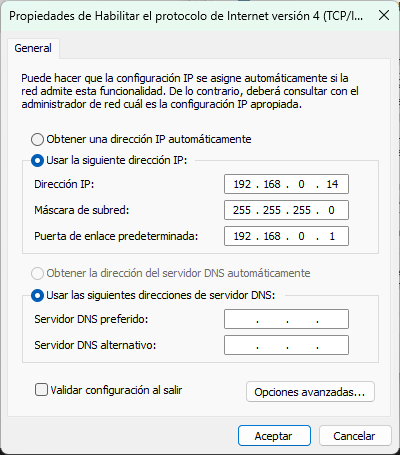
\includegraphics[width=0.6\textwidth]{img/cambiar_IP_Windows.png}
            \caption{Configuración de la Dirección IP en Windows}
            \label{fig:ip_windows}
        \end{figure}

        Para obtener la dirección MAC de un equipo en Windows abrimos la terminal y ejecutamos el comando \texttt{ipconfig -all} y se mostrará la dirección MAC como se muestra en la Figura~\ref{fig:mac_windows}. La dirección MAC que se obtuvo de la PC1 fue \texttt{64:00:6A:44:B6:0A}.

        \begin{figure}[H]
            \centering
            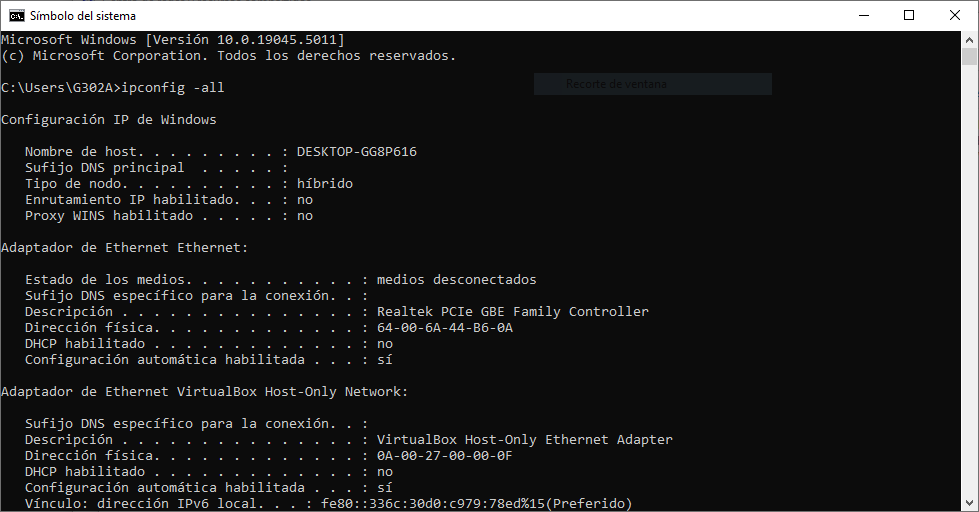
\includegraphics[width=0.6\textwidth]{img/direccion_MAC_windows.PNG}
            \caption{Obtención de la Dirección MAC en Windows}
            \label{fig:mac_windows}
        \end{figure}

        En la PC2 se inició con el sistema operativo \textbf{Linux} y se realizó el cambio de la dirección IP a \texttt{192.168.0.13} con la puerta de enlace \texttt{192.168.0.1}. Como se muestra en la Figura~\ref{fig:ip_linux}.

        \begin{figure}[H]
            \centering
            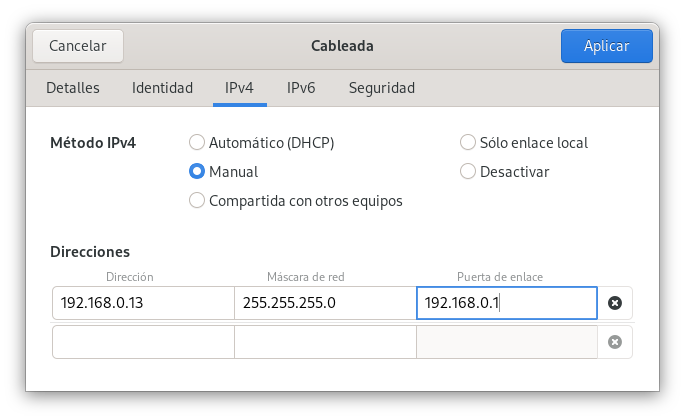
\includegraphics[width=0.6\textwidth]{img/cambiar_IP_Linux.png}
            \caption{Configuración de la Dirección IP en Linux}
            \label{fig:ip_linux}
        \end{figure}

        Para obtener la dirección MAC en la PC2 con Linux nos dirigimos a configuración de red y seleccionamos la interfaz de red deseada, en este caso \textbf{Ethernet} y se mostrará la dirección MAC como se muestra en la Figura~\ref{fig:mac_linux}. La dirección MAC que se obtuvo de la PC2 fue \texttt{64:00:6A:44:A5:DF}.
        \begin{figure}[H]
            \centering
            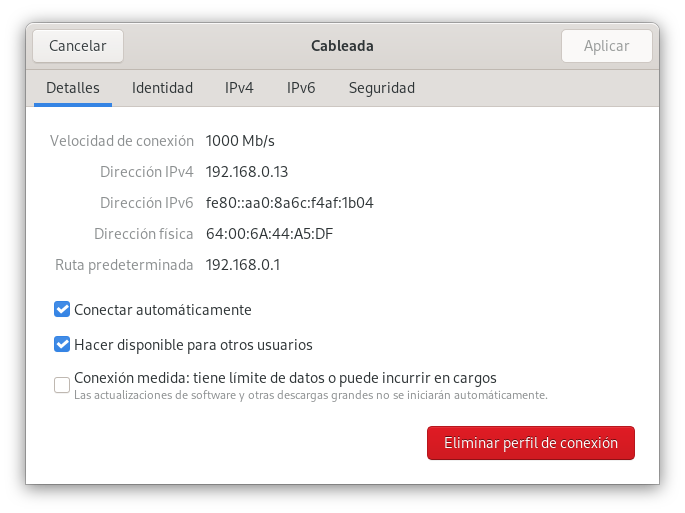
\includegraphics[width=0.6\textwidth]{img/direccion_MAC_linux.png}
            \caption{Obtención de la Dirección MAC en Linux}
            \label{fig:mac_linux}
        \end{figure}

        Los datos obtenidos de ambas PC's se muestran en el Cuadro~\ref{tab:tabla_equipos}.

        \begin{table}[H]
            \centering
            \begin{tabular}{c|c|c|c}
                \textbf{Integrante} & \textbf{Equipo} & \textbf{IP} & \textbf{MAC} \\
                \hline
                Diego Alexis Moreno Valero & PC1 & 192.168.0.14 & 64:00:6A:44:B6:0A \\
                Luis Ángel Cruz Díaz & PC2 & 192.168.0.13 & 64:00:6A:44:A5:DF \\
            \end{tabular}
            \caption{Tabla de Equipos}
            \label{tab:tabla_equipos}
        \end{table}
    \subsection{Tarea 2.}
        \paragraph{Paso 1.}
        Tabla ARP.
        \begin{enumerate}
            \item \textbf{Borre el contenido de la tabla ARP.}\\
            Para borrar la tabla ARP de la PC1, debemos abrir la terminal de Windows y ejecutamos el comando \texttt{arp -d} como se muestra en la Figura~\ref{fig:borrar_arp}. No se muestra la ejecución del comando ya que no se obtiene una respuesta del sistema.
            \begin{figure}[H]
                \centering
                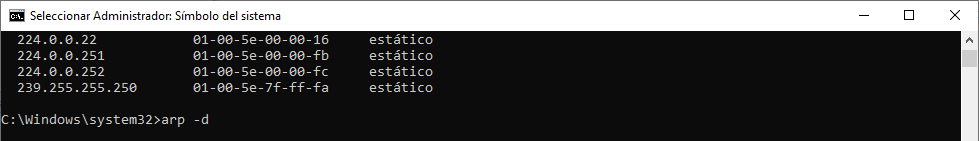
\includegraphics[width=0.6\textwidth]{img/borrar_tabla_ARP.PNG}
                \caption{Borrar Tabla ARP}
                \label{fig:borrar_arp}
            \end{figure}
            \item \textbf{Muestre el contenido de la tabla ARP.}\\
            Para mostrar la tabla ARP de la PC1, debemos abrir la terminal de Windows y ejecutamos el comando \texttt{arp -a} como se muestra en la Figura~\ref{fig:tabla_arp}.
            \begin{figure}[H]
                \centering
                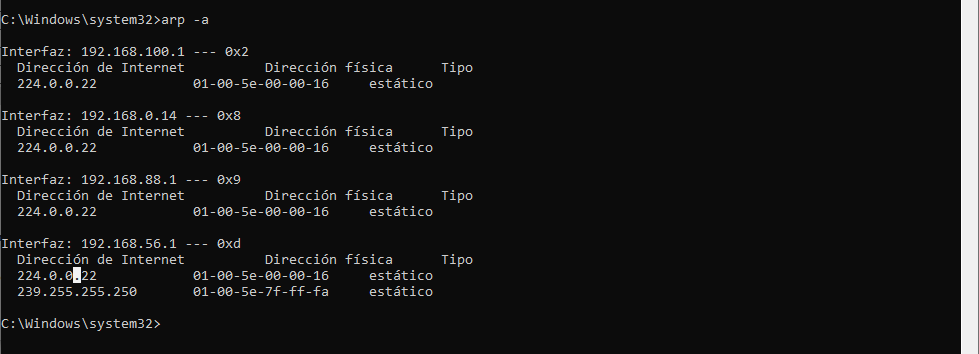
\includegraphics[width=0.6\textwidth]{img/tabla_ARP.PNG}
                \caption{Tabla ARP}
                \label{fig:tabla_arp}
            \end{figure}
            \item \textbf{¿Qué comandos y qué parametros se empleó en los puntos (a) y (b)?}
            \begin{enumerate}
                \item En el punto (a) se empleó el comando \texttt{arp} con el parámetro \texttt{-d} para borrar la tabla ARP. 
                \item En el punto (b) se empleó el comando \texttt{arp} con el parámetro \texttt{-a} para mostrar la tabla ARP.
            \end{enumerate}
            \item \textbf{Explique con detalle el contenido de la tabla.}\\
            Podemos observar en la Figura~\ref{fig:tabla_arp} que la tabla ARP contiene la dirección IP y la dirección MAC de los equipos que han sido contactados recientemente por la PC1.
        \end{enumerate}

    \subsection{Tarea 3.}
        \paragraph{Paso 1.}
        Arranquen en la PC1 \textbf{Wireshark} para capturar el tráfico en su interfaz ethernet empleando los filtros adeacuados (ARP).
        \paragraph{Paso 2.}
        Realice el ping de la PC2 a la PC1.
        \begin{enumerate}
            \item ¿Cuál es el comando y los parámetros empleados?\\
            Una vez terminado el ping, interrumpan la captural del Wireshark y guarde la captura en un archivo (utilicen como nombre del archivo captura1.cap)
            Compruebe el estado de las cachés del ARP en la PC.
            \item Consulte la tabla ARP y analice si hubo cambios con los valores obtenidos en el paso 1 de la tarea 2; explique el contenido de la tabla.
        \end{enumerate}
        \paragraph{Paso 3.}
        Configure los filtros para capturar toda la información que se genere. Envíe el ping de la PC2 a la PC1 y al finalizar guarde el archivo como captura2.cap.
    \subsection{Tarea 4.}
        \paragraph{Paso 1.}
        Con Wireshark cargue cada archivo capturado y explique los resultados obtenidos.

\section{Conclusiones}

% --- Para agregar un apéndice
%\newpage
%\appendix
%\appendixpage
%\addappheadtotoc
%\section{Nombre del apéndice}